\documentclass[a4paper, 12pt]{scrartcl}

\usepackage[utf8]{inputenc}
\usepackage[T1]{fontenc}
\usepackage[ngerman]{babel}

\usepackage{amssymb}
\usepackage{amsmath}
\usepackage{physics}
\usepackage{framed}
\usepackage{float}
\usepackage{mathtools}
\usepackage{marvosym}
\usepackage{bbm}

\usepackage{tikz}
\usepackage{chngcntr}

\usepackage{amsthm}
\usepackage{thmtools}

\usepackage[left=2cm, right=2cm, top=2cm]{geometry}

\allowdisplaybreaks

\setlength{\parindent}{0pt}

\setkomafont{paragraph}{\normalfont\itshape}


\declaretheoremstyle[%
  spaceabove=0,%
  spacebelow=6pt,%
  headfont=\normalfont\itshape,%
  postheadspace=1em,%
  headpunct={}
]{mystyle}

\declaretheorem[name={Behauptung}, style=mystyle, unnumbered]{theorem}
\declaretheorem[name={Lemma}, style=mystyle]{lemma}
\declaretheorem[name={Voraussetzung}, style=mystyle, unnumbered]{precondition}
\let\proof\oldproof
\declaretheorem[name={Beweis}, style=mystyle, qed=\qedsymbol, unnumbered]{proof}

\newcounter{taski}
\newcounter{taskii}[taski]
\newcounter{taskiii}[taskii]

\newcommand{\task}{\stepcounter{taski}\textbf{Aufgabe \arabic{taski}}~}
\newcommand{\ttask}{\stepcounter{taskii}\textbf{(\alph{taskii})}~}
\newcommand{\tttask}{\stepcounter{taskiii}\quad(\roman{taskiii})~}

\setcounter{taski}{12}
\begin{document}
\begin{center}
    \textbf{4. Abgabeblatt}\\[2em]
	\def\arraystretch{2}
    \begin{tabular}{|l|l|l|l||p{18mm}|}
        \hline
        Aufgabe 13 & Aufgabe 14 & Aufgabe 15 & Aufgabe 16 & Summe:~ \\
        \hline &&&&\\
         \hline  
    \end{tabular}
\end{center}
\begingroup
\def\arraystretch{1.5}
\begin{tabular}{p{.5\textwidth}p{.5\textwidth}}
	\hline
    Übungsgruppe: Mo 14:15 ~~ SR B& Tutor(in): Sebastian Groß\\
    Namen: Ellen Bräutigam, Kamal Abdellatif &\\
    \hline
\end{tabular}
\endgroup\\

\task
\ttask
Nach dem \textsc{Sylvester}'schen Trägheitssatz existiert eine Matrix $T \in \mathrm{GL}(n,\,\mathbb{R})$ sodass
\[ T^\top AT = \mqty(\diagonalmatrix{E_p, -E_q, 0}) \qquad p,\,q \in \mathbb{N} \qc p+q \leq n \]
Man wähle als Basis $\mathcal{B} = (b_1,\,\dots,\,b_n)$ die Spalten von $T$. Diese bilden eine Matrix, da $T$ vollen Rang besitzen muss. Es folgt mit $\Phi_\mathcal{B} = \widetilde{T}$
\begin{align*}
    (Q \circ \Phi_ \mathcal{B})(y) = (Ty)^\top A (Ty) &= y^\top (T^\top A T) y = \mqty(y_1 & \cdots & y_n) \mqty(\diagonalmatrix{E_p, -E_q, 0}) \mqty(y_1 \\ \vdots \\ y_n) \\
    &= \sum_{j=0}^p y_j^2 - \sum_{j=p+1}^{p+q} y_i^2
\end{align*}
\ttask
\begin{gather*}
    \mqty(1 & -1 \\ -1 & 0) \quad \rightarrow \quad \mqty(1 & 0 \\ 0 & -2) \quad \rightarrow \quad \mqty(1 & 0 \\ 0 & -1) \\
    \mqty(1 & -1 \\ -1 & 1) \quad \rightarrow \quad \mqty(1 & 0 \\ 0 & -1) \\
    \mqty(1 & -1 \\ -1 & 3) \quad \rightarrow \quad \mqty(1 & 0 \\ 0 & 1) \qc T = \mqty(1 & \frac{\sqrt{2}}{2} \\ 0 & \frac{\sqrt{2}}{2}) \qc \mathcal{B} = \qty((1,\,0)^\top,\,\frac{1}{2}(\sqrt{2},\,\sqrt{2})^\top)
\end{gather*}
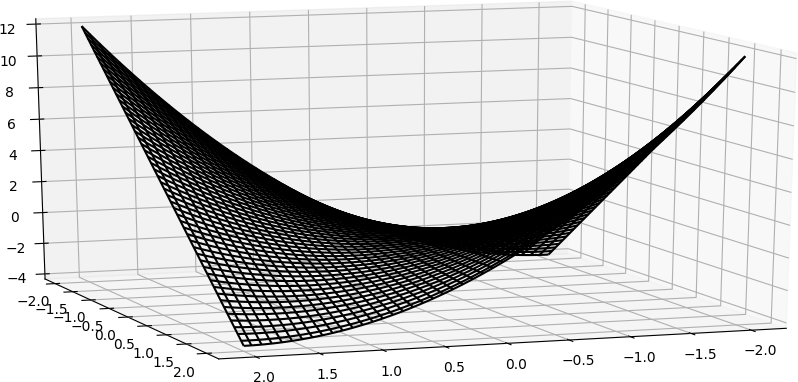
\includegraphics[width=.33\textwidth]{1.png}\hfill
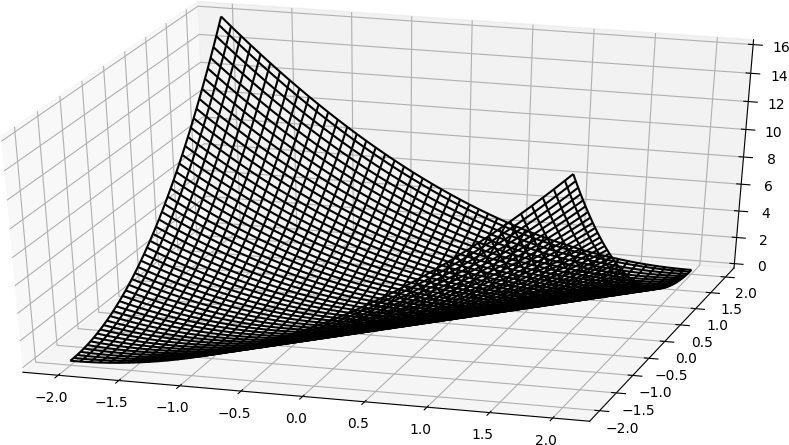
\includegraphics[width=.33\textwidth]{2.png}\hfill
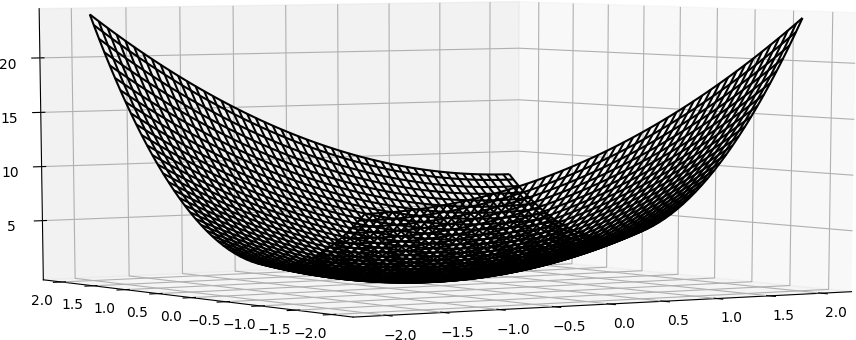
\includegraphics[width=.33\textwidth]{3.png}
\end{document}
